% !TEX root = knottedMain.tex
\documentclass[varwidth=\maxdimen]{standalone}

\usepackage{mathtools,amssymb,mathrsfs,dutchcal,upgreek,faktor,accents,etoolbox,multicol}
\usepackage[dvipsnames]{xcolor}
\definecolor{mygreen}{RGB}{	8,156,79 }
\usepackage{tikz,tikz-cd}
\usetikzlibrary{patterns,knots,arrows.meta,decorations.markings}
\tikzset{>={Straight Barb[scale=0.85]}}
\tikzcdset{
  cells={font=\everymath\expandafter{\the\everymath\displaystyle}},
  arrow style=tikz,
  diagrams={>={Straight Barb[scale=0.85]}},
  every label/.append style = {font = \small}
}


\begin{document}
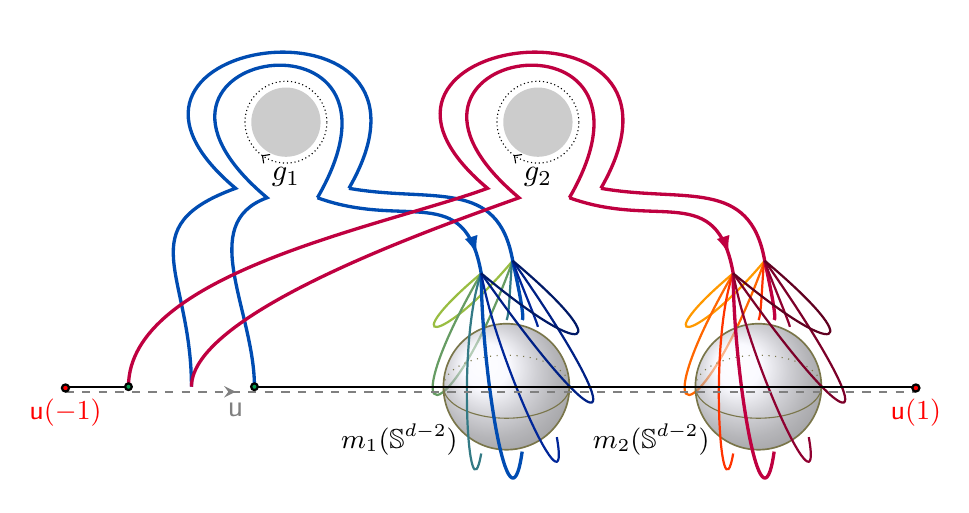
\begin{tikzpicture}[scale=0.8,every node/.style={scale=1.1},even odd rule]
    \clip (1.4,-1.55) rectangle (15.9,5.7);
\foreach \y/\c in {9/blue!65!green,13/red}{
        % the leftmost
        \draw[\c!40!yellow,  thick]
                (\y-.4,1.8) to[out=-140,in=-130, distance=1.8cm] (\y+.1,2);
        %the second from left
        \draw[\c!60!yellow,  thick]
                (\y-.4,1.8) to[out=-120,in=-110, distance=3cm] (\y+.1,2);
        % spheres
            \shade[ball color=blue!5!white,opacity=0.55] (\y,0) circle (1cm);
            \draw[black!60!yellow] (\y-1,0) arc (180:360:1cm and 0.5cm);
            \draw[black!60!yellow,dotted] (\y-1,0) arc (180:0:1cm and 0.5cm);
            \draw[black!60!yellow,semithick] (\y,0) circle (1cm);
    }
    \foreach \y/\c/\rc/\mid/\i in {9/blue!65!green/blue!80!green/blue!70!green/1,
    13/red/purple/purple/2}{
    % the third from left
    \draw[\c!80!yellow, thick]
            (\y-.4,1.8) to[out=-110,in=-100, distance=1.15cm] (\y-.4,-1.06)
            (\y,1.06) to[out=40,in=-120, distance=0.07cm] (\y+.1,2);

    \draw[\mid, very thick,postaction=decorate,decoration = {markings, mark = at position 0.9 with {\arrow{latex}} }]
            (\y+-3,3) to[out=-20,in=100, distance=1.5cm]
            (\y-.4,1.8);
    % middle end
    \draw[\mid, very thick]
            (\y-.4,1.8) to[out=-90,in=-98, distance=1.5cm]
            (\y+.25,-1.03)
            (\y+.25,1.06) to[out=40,in=-80, distance=0.07cm]
            (\y+.1,2) to[out=100,in=-10, distance=1.35cm] (\y-2.5,3.15);
    % gp element and middle start
    \draw[\mid, very thick]
                    (5-\i,0) to[out=90,in=-160, distance=1.8cm]
                    (\y-5+.7,3.15) to[out=140,in=60, distance=3.8cm]
                    (\y-2.5,3.15)

                    (6-\i,0) to[out=90,in=-160, distance=1.2cm]
                    (\y-4+.2,3) to[out=140,in=60, distance=3.7cm]
                    (\y-3,3) ;
    % the grey hole
    \fill[color=black!20!white] 
        (\y-3.5,4.2) circle (0.55cm);
    \draw[black,densely dotted,postaction = decorate,decoration = {markings, mark = at position 0.65 with {\arrowreversed{>}} }] 
        (\y-3.5,4.2) circle (0.65cm) node[below=0.4cm]{$g_{\i}$};
    % the third from right
    \draw[\rc!75!black,  thick]
            (\y-.4,1.8) to[out=-80,in=-80, distance=1.4cm] (\y+.8,-0.8)
            (\y+.5,0.95) to[out=100,in=-80, distance=0.1cm] (\y+.1,2);
    % the second from right
    \draw[\rc!65!black, thick]
           (\y-.4,1.8) to[out=-55,in=-55, distance=3.5cm] (\y+.1,2);
    % the rightmost
    \draw[\rc!50!black, thick]
            (\y-.4,1.8)to[out=-40,in=-40, distance=2.2cm] (\y+.1,2);
    }
    \draw[gray,thick, dashed,postaction=decorate,decoration = {markings, mark = at position 0.2 with {\arrow{stealth}}}]
            (2,-0.08) -- (15.5,-0.08) node[below,pos=0.2]{$\mathsf{u}$};
    \draw[thick]
        (2,0) -- (3,0) 
        (5,0) -- (15.5,0) 
        (7.3,0) node[below=0.3cm]{\small$m_1(\mathbb{S}^{d-2})$}
        (11.3,0) node[below=0.3cm]{\small$m_2(\mathbb{S}^{d-2})$};
    % \draw[mygreen, -latex, very thick]
    %     (4,0) -- (5,0) node[pos=0.5,below=2pt]{$J_0$};

    \fill[mygreen,draw=black,thick] 
        (3,0) circle (1.5pt) 
        (5,0) circle (1.5pt);
    \fill[red,draw=black,thick]
        (2,-0.02) circle (1.6pt) 
        node[below]{\small$\mathsf{u}(-1)$}
        (15.5,-0.02) circle (1.6pt) 
        node[below]{\small$\mathsf{u}(1)$};
\end{tikzpicture}

    % \vspace{-10pt}
\end{document}